
\subsection{Etat de l'art des modèles}

Vous pourrez trouver un recensement des références de modèles et de dataset (paper et code) sur ce répertoire github \cite{state_of_the_art_crowd_counting}. Beaucoup de modèles existent déjà pour la détection des têtes, mais pour ce projet et pour apprentissage nous avons décidé d'utiliser YOLOv11 \cite{khanam2024yolov11overviewkeyarchitectural}, avec un finetuning sur notre dataset d'images.

ILANN BLABLABLA

\subsection{Datasets}

Il existe plusieurs datasets pour la détectiond des têtes et avec l'utilisation grandissante des cameras comme moyens de surveillance, ils se sont multipliés et sont de plus en plus gros. On dispose donc de beaucoup de matériel pour notre entrainement et évaluation, certains articles \cite{state_of_the_art_datasets} proposent des benchmarks pour les datasets les plus utilisés.

Pour notre utilisation, nous cherchons des datasets avec un nombre de personne supérieur à 100, car nous souhaitons nous intérresser spécifiquement aux foules denses. Pour cela nous avons sélectionnés les datasets JHU-Crowd++ \cite{sindagi2020jhu-crowd++} (le seul utilisé dans ce projet en réalité) qui présente 4372 avec en moyenne 346 personnes et jusque 25,791.
Nous avons selectionné 2 autres datasets semblables que nous n'avons pas utilisé dans ce projet, le NWPU-Crowd \cite{gao2020nwpu} avec 5,109 images d'en moyenne 418 personnes, et le UCF-QNRF \cite{idress2018ucfqnrf} avec 1,535 images d'en moyenne 815 personnes.

\subsection{Finetuning}

ILANN BLABLABLA

\subsection{Résultats qualitatifs}

Comme vous pouvez le voir sur l'exemple Figure \ref{fig:heads-detection}, la détection des têtes est plutôt bonne, lorsque l'on est dans les champs proches et/ou que l'on voit bien l'entièreté de la tête.

Cependant le modèle atteint ses limites lorsqu'il y a beaucoup de têtes sur l'image, ou que celles-ci sont partiellement caché ou en mauvaise résolution (car trop loin)
.
\begin{figure}[h!]
    \centering
    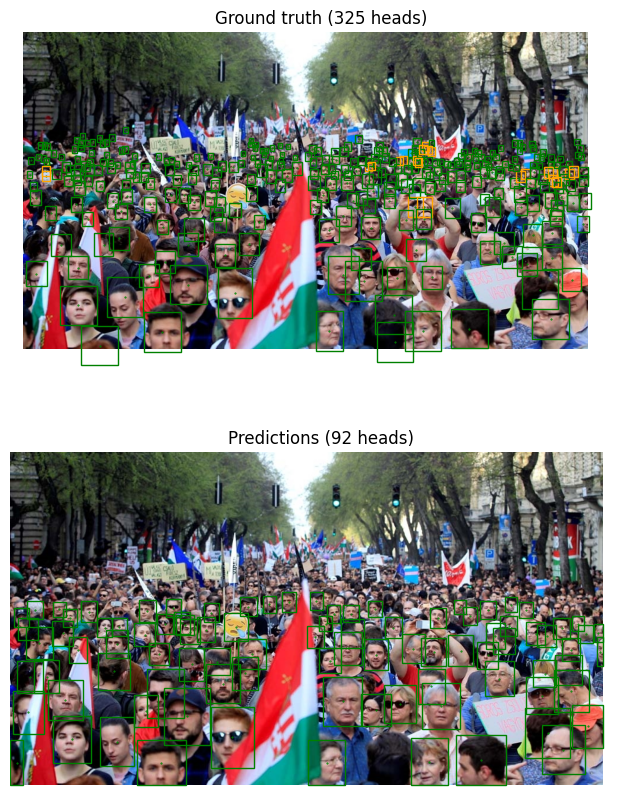
\includegraphics[width=0.45\textwidth]{images/heads_detection.png}
    \caption{Résultats qualitatif de la détection des têtes.}
    \label{fig:heads-detection}
\end{figure}